\documentclass[a4paper,12pt]{article} 

%Выравнивание названия таблиц по левому краю
%\usepackage[nooneline]{caption} 
%Размеры отступов 
\usepackage[left=20mm, top=20mm, right=20mm, bottom=20mm, footskip=10mm]{geometry}

%Рисунки
\usepackage{graphicx}
\usepackage{wrapfig}

%Русский язык в формулах
\usepackage{mathtext}

%  Русский язык
\usepackage[T2A]{fontenc}			
\usepackage[utf8]{inputenc}			
\usepackage[english,russian]{babel}	

%Готические буквы
\usepackage{amssymb}

% Математика
\usepackage{amsmath,amsfonts,amssymb,amsthm,mathtools} 
\usepackage{wasysym}

\begin{document} 

%Титульник 
\begin{titlepage}
	\begin{center}
		\large 	МИНИСТЕРСТВО ОБРАЗОВАНИЯ И НАУКИ РОССИЙСКОЙ ФЕДЕРАЦИИ\\
				МОСКОВСКИЙ ФИЗИКО-ТЕХНИЧЕСКИЙ ИНСТИТУТ \\
				(НАЦИОНАЛЬНЫЙ ИССЛЕДОВАТЕЛЬСКИЙ ИНСТИТУТ)\\ 
				ФИЗТЕХ-ШКОЛА ЭЛЕКТРОНИКИ, ФОТОНИКИ \\
				И МОЛЕКУЛЯРНОЙ ФИЗИКИ \\
		
		
		\vspace{4.0 cm}
		Лабораторная работа № 3.1.3 \\ 
		\LARGE \textbf{Измерение магнитного поля Земли}
	\end{center}
	\vspace{3 cm} \large
	
	\begin{flushright}
		выполнил студент 2 курса \\
		{группы Б04-006}\\
		\textbf{Белостоцкий Артемий}\\
	\end{flushright}
	
	\vfill

	\begin{center}
	Долгопрудный, 2021 г.
	\end{center}
\end{titlepage}                                                                      
 
\section{Цель работы}
Исследовать свойства постоянных неодимовых магнитов;
измерить с их помощью горизонтальную и вертикальную составляющие
индукции магнитного поля Земли и магнитное наклонение.


\section{В работе используются}
	\begin{itemize}
	\item Неодимовые магниты;
	\item Тонкая нить для изготовления крутильного маятника;
	\item Медная проволока
	\item Электронные весы;
	\item Секундомер;
	\item Измеритель магнитной индукции;
	\item Штангенциркуль;
	\item Брусок, линейка
и штатив из немагнитных материалов;
	\item Набор гирь и разновесов;
	\end{itemize}


\section{Теоретические сведения}
\subsection*{Точечный магнитный диполь}
Простейший магнитный диполь может быть образован витком с током или постоянным магнитом. По определению, магнитный момент $\mathfrak{m}$ тонкого витка площадью $S$ с током $I$ равен
$$
{\mathfrak{m}}=\dfrac{I}{c}\vec{S}=\dfrac{I}{c}S\vec{n},
$$
где $\vec{S}=S\vec{n}$ -- вектор площади круга контура. Если размеры контура с током или магнитной стрелки малы по сравнению расстоянием до диполя, то соответствующий магнитный диполь называют элементарным или точечным.\\
Магнитное поле точечного диполя определяется по формуле, аналогичной формуле для поля
элементарного электрического диполя:
$$
\vec{B}=\dfrac{3(\mathfrak{m},\vec{r})\vec{r}}{r^5} - \dfrac{\mathfrak{m}^2}{r^3}
$$ 
В магнитном поле с индукцией $B$
на точечный магнитный диполь 
действует механический
момент сил:
$$
\vec{M} = {\mathfrak{m}}\times \vec{B}.
$$
Под действием вращающего момента $\vec{M}$ виток с током или постоянный магнит поворачивается
так, чтобы его магнитный момент выстроился вдоль вектора индукции магнитного поля. Это —
положение устойчивого равновесия: при отклонении от этого положения возникает механический
момент внешних сил, возвращающий диполь к положению равновесия. В положении, когда ${\mathfrak{m}}$ и $\vec{B}$
параллельны, но направлены противоположно друг другу, также имеет место равновесие ($M$ = 0),
но такое равновесие неустойчиво: малейшее отклонение от этого положения приведёт к появлению
момента сил, стремящихся отклонить диполь ещё дальше от начального положения.\\
Магнитный диполь в магнитном поле обладает энергией:
$$
W = -({\mathfrak{m}},\vec{B})
$$
В неоднородном поле на точечный магнитный диполь, кроме момента сил, действует ещё и сила:
$$
\vec{F}=({\mathfrak{m}},\vec{\triangledown})\vec{B}
$$
Используя формулы для момента силы, силы и энергии, не сложно выяснить, как ведёт себя
свободный магнитный диполь в неоднородном магнитном поле: он выстраивается вдоль силовых
линий магнитного поля и, кроме того, под действием результирующей силы, возникающей из-за
неоднородности поля, втягивается в область более сильного магнитного поля, т.е. в область, где он
обладает меньшей энергией.\\
Зная магнитные моменты $\mathfrak{m}_1 = \mathfrak{m}_2 = \mathfrak{m}$ двух небольших постоянных магнитов, можно рассчитать силу
их взаимодействия:
$$
F = \mathfrak{m} \dfrac{\partial B}{\partial r}=-6\dfrac{\mathfrak{m}^2}{r^4}.
$$


\section{Экспериментальная установка}

В работе используются неодимовые магниты шарообразной формы 

Для проведения эксперимента важно, что а) вещество, из которого
изготовлены магниты, является \textit{магнитожёстким} материалом; б) шары намагничены однородно.  

Магнитное поле однородно намагниченного шара радиусом R может быть вычислено точно. На расстояниях r > R от центра шара оно совпадает с полем точечного магнитного диполя (2), расположенного в центре, магнитный момент $\mathfrak{m}$ которого совпадает с полным моментом шара. Внутри шара магнитное поле однородно: c помощью условия непрерывности нормальной компоненты индукции на поверхности шара нетрудно получить, что при r < R:

\begin{equation}
	\mathbf{B_0} = \dfrac{2 \mathfrak{m}}{R^3}
\end{equation}

В качестве ещё одной характеристики материала магнита используют остаточную \textit{намагниченность} \textbf{M}. По определению, намагниченность \textit{равна объёмной плотности магнитного момента},поэтому для однородно намагниченного шара
	
\begin{equation}
	\mathfrak{m} = \mathbf{M} V,
\end{equation}

где $V = \frac{4\pi}{3} R^3$ объём магнита. Величину $\textbf{B}_r = \mu_0 \textbf{M}$ называют \textit{статочной индукцией материала}

Из (2) нетрудно видеть, что индукция $\textbf{B}_p$ на полюсах однородно намагниченного шара направлена по нормали к поверхности и совпадает
поэтому с индукцией внутри шара $\textbf{B}_p$ = $\textbf{B}_0$. Как следует из (1), величина $\textbf{B}_p$ связана с остаточной индукцией $\textbf{B}_0$ соотношением:

\begin{equation}
	\overrightarrow{B_p} = \overrightarrow{B_0} = \dfrac{2}{3} \overrightarrow{B_r}
\end{equation}

\newpage

\subsection*{Определение магнитного момента магнитных шариков}

\begin{wrapfigure}{l}{5 cm}
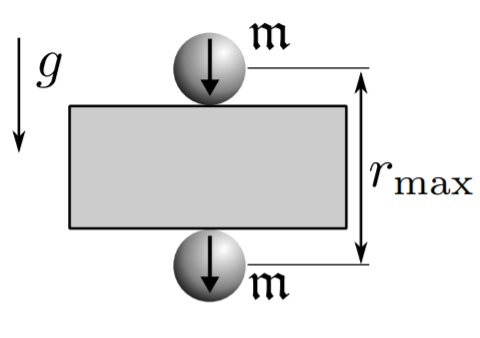
\includegraphics[width = 5 cm]{fig1}
\caption{Измерение магнитных моментов шариков}
\end{wrapfigure}

\textbf{Метод А}. Величину магнитного момента $\mathfrak{m}$ двух
одинаковых шариков можно рассчитать, зная их
массу m и определив максимальное расстояние $r_{max}$,
на котором они ещё удерживают друг друга в поле
тяжести (см. рис. 1). При максимальном расстоянии
сила тяжести шариков mg равна силе их магнитного
притяжения. Когда векторы двух магнитных моментов ориентированы вертикально, из (6) имеем

\begin{equation}
	\mathfrak{m} = \sqrt{\frac{mgr^4_{max}}{6}}
\end{equation}

По величине $\mathfrak{m}$ можно рассчитать величину индукции B вблизи любой точки на поверхности шара радиуса R. Максимальная величина индукции наблюдается на полюсах.


\begin{wrapfigure}{r}{5 cm}
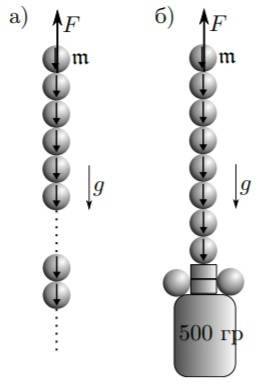
\includegraphics[width = 5 cm, height = 6 cm]{fig2}
\caption{Альтернатиный метод Измерения магнитных моментов шариков}
\end{wrapfigure}

\vspace{0.3 cm}

\textbf{Метод B}. Величину магнитного момента шариков можно определить также по силе их сцепления. Она определяется как сила, необходимая для разрыва двух сцепившихся магнитных шариков. Сила сцепления
максимальна, если шары соединяются своими противоположными полюсами (магнитные моменты сонаправлены).

Максимальную силу сцепления можно
определить по весу магнитной цепочки, которую способен удержать самый верхний магнитный шарик. Если цепь состоит из одинаковых магнитных шариков (см. рис. 2а), то при определённой длине она отрывается от верхнего шарика

Сила сцепления двух одинаковых шаров радиусами R с магнитными моментами $\mathfrak{m}$ равна

\begin{equation}
	F_0 = \frac{3 \mathfrak{m}^2}{8R^4} \label{force}
\end{equation}

Тогда минимальный вес цепочки, при которой она оторвётся от верхнего шарика, равен

\begin{equation}
F \approx 1,08 F_0
\end{equation}

\newpage

\subsection*{Измерение горизонтальной составляющей индукции магнитного поля Земли}

\begin{wrapfigure}{l}{5 cm}
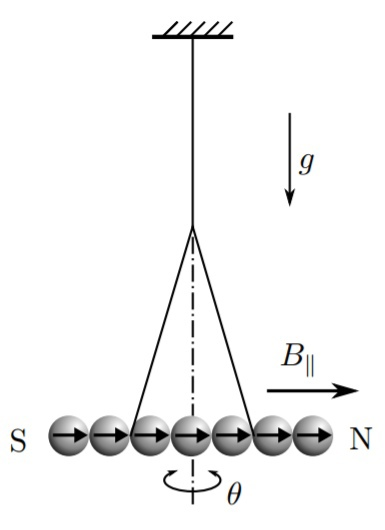
\includegraphics[width = 5 cm, height = 7 cm]{fig3}
\caption{Измерение магнитных моментов шариков}
\end{wrapfigure}

Магнитное поле Земли в настоящей работе измеряется по периоду
крутильных колебаний <<магнитной стрелки>> вокруг вертикальной оси.

<<Магнитная стрелка>> образована сцепленными друг с другом n намагниченными
шариками. С помощью $\Lambda$ -- образного подвеса
стрелка подвешена в горизонтальном положении (см. рис. 3). Для крепления нити в
работе используется штатив, изготовленный
из немагнитного материала.

Магнитные моменты всех шариков направлены в одну сторону вдоль оси <<стрелки>>. Под действием механического момента
сил, действующего на стрелку со стороны
поля Земли, стрелка стремится повернуться
по горизонтальной составляющей магнитного поля Земли $B_{||}$ в направлении Юг—Север.

При отклонении стрелки на угол $\theta$ от равновесного положения в горизонтальной плоскости возникают крутильные колебания вокруг вертикальной оси, проходящей через середину стрелки. Если пренебречь упругостью нити, то уравнение крутильных колебаний такого
маятника определяется возвращающим моментом сил.

\begin{equation}
	M = - \mathfrak{m}_n B_{||} \sin \theta
\end{equation}

и моментом инерции $J_n$ <<стрелки>> относительно оси вращения. При малых амплитудах ($\sin \theta \approx \theta$) уравнение колебаний стрелки имеет вид

\begin{equation}
	J_n \ddot{\theta} + \mathfrak{m}_n B_{||} \theta = 0.
\end{equation}

Отсюда находим период малых колебаний:

\begin{equation}
	   T = 2\pi \sqrt{ \frac{J_n}{\mathfrak{m}_n B_{||}} }
\end{equation}

Здесь $\mathfrak{m}_n$ = n\textbf{m} — полный магнитный момент магнитной <<стрелки>>,
составленной из n шариков. Момент инерции $J_n$ стрелки из n шариков с
хорошей точностью равен моменту инерции тонкого однородного стержня массой $m_n$ = nm и длиной $l_n$ = n * 2R.

\newpage

\subsection*{Измерение вертикальной составляющей индукции магнитного поля Земли. Магнитное наклонение.}

Для измерения вертикальной $B_{\perp}$ составляющей вектора индукции
поля Земли используется та же установка, что и для измерения горизонтальной составляющей с тем лишь отличием, что подвешенная магнитная <<стрелка>> закрепляется на нити в одной точке. В этом случае
стрелка, составленная из чётного числа одинаковых шариков и подвешенная за середину, расположится не горизонтально, а под некоторым
углом к горизонту (см. рис. 4а). Это связано с тем, что вектор B индукции магнитного поля Земли не горизонтален, а образует с горизонтом
некоторый угол $\beta$, зависящий от географической широты $\varphi$ места, где
проводится опыт. Величина угла $\beta$ называется магнитным наклоном

\begin{figure}[h]
	\begin{center}
	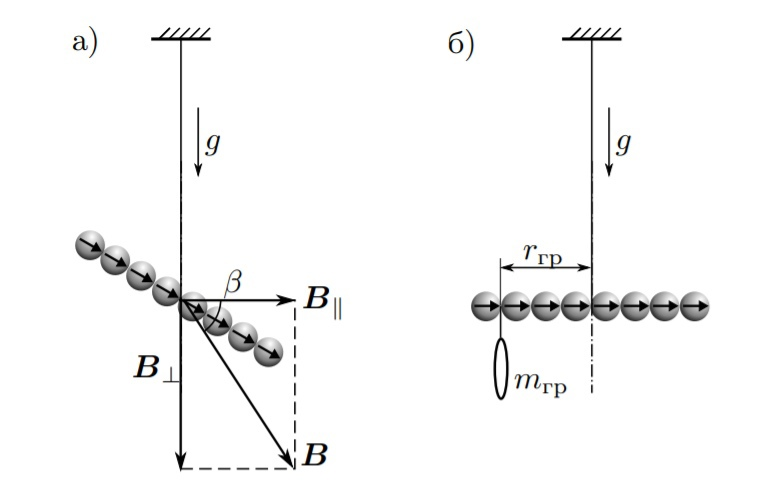
\includegraphics[scale=0.5]{fig4}
	\end{center}
	\caption{Измерение вертикальной составляющей поля и магнитного наклонения}
`\end{figure}

Измерить магнитное наклонение непосредственно по положению подвешенной <<стрелки>> затруднительно из-за механического момента нити
в точке подвеса, неизбежно возникающем при наклоне <<стрелки>>. Избавиться от этого можно, если выровнять её горизонтально с помощью небольшого дополнительного грузика (см. рис. 4б). В этом случае момент силы тяжести груза относительно точки подвеса будет равен моменту сил, действующих на <<стрелку>> со стороны вертикальной составляющей магнитного поля Земли. Если масса уравновешивающего груза равна $m_w$, плечо силы тяжести $r_w$ а полный магнитный момент стрелки $\mathbf{m}_n$ = n * \textbf{m}, то в равновесии

\begin{equation}
	M_n = m_{w}gr_{w} = n \mathfrak{m}B_{\perp}
\end{equation}

\newpage

\section{Ход работы}

\subsection*{Задание №1}

\subsubsection*{Метод А}

Взвесим n = 13 шариков на весах и определим среднее значение массы и среднеквадратичное отклонение по формуле:

$$
	\sigma = \sqrt{\frac{1}{n(n-1)}\sum_{i=1}^n(m_i - m)^2}
$$
\vspace{0.5 cm}
Получим:
\vspace{0.0 cm}
$$
	m = 0,485 \pm 0,003 \ г
$$

Аналогично определим диаметр шариков. Получим:
$$
	d = 0,494 \pm 0,017 \ см 
$$

Проложим между двумя шариками книгу. Увеличивая расстояние между магнитами (добавляя листы бумаги) выясним,  на каком максимальном расстоянии $r_{max}$ шарики удерживают друг друга в поле тяжести Земли. Для 6 пар шариков, аналогично предыдущим рассуждениям, получим:

$$
	r_{max} = 1,57 \pm 0,07 см
$$

Рассчитаем величину магнитного момента магнитика $\mathfrak{m}$, прировняв силу притяжение двух магнитных диполей \eqref{force} силе тяжести $F_т = mg$:

$$
	\mathfrak{m} = \sqrt{\frac{mgr^4_{max}}{6}} \approx 21,92 \ Гс*см^3
$$

Погрешность для $\mathfrak{m}$ найдем по формуле:

$$
	\sigma_{\mathfrak{m}} = \mathfrak{m} \sqrt{ \frac{1}{4}  \frac{\sigma_m^2}{m^2} + 4 \frac{\sigma_{r_{max}} ^2}{r_{max}^2}} \approx 2,08 \ Гс*см^3
$$

Тогда намагниченность шара:

$$
	M = \frac{6\mathfrak{m}}{\pi d^3} \approx 347,54 \ Гс	
$$

Погрешность для M найдем по формуле:

$$
	\sigma_M = M\sqrt{\frac{\sigma_{\mathfrak{m}}^2}{\mathfrak{m}^2} + 9\frac{\sigma_d^2}{d^2}} \approx 49,30 \ Гс
$$

По величине намагниченности рассчитаем поле на полюсах шарика:

$$
	B_p = \frac{8\pi}{3}M \approx 2911 \ Гс
$$
$$	
	\sigma_{B_p} = B_p \frac{\sigma_M}{M} \approx 413 \ Гс
$$

Окончательно:

$$
	B_p = 2911 \pm 413 \ Гс
$$

\newpage

Рассчитаем величину остаточной магнитной индукции материала, из которого изготовлен магнитный шарик:

$$
	B_r = 4\pi M \approx 4367 \ Гс
$$


\subsubsection*{Метод Б}

Составим цепочку из 20 шариков и, с помощью неодимовых магнитов в форме параллелепипедов, подсоединим цепочку к гире и разновесам.Добавляя шарики, подберем минимальный вес F системы с цепочкой и гирей, при котором она открывается от верхнего шарика:

$$
	F = 2,184 \ Н = 218,4 \ кДин
$$

Определим силу сцепления двух шаров:

$$
	F_0 = \frac{F}{1,08} \approx 202,2 \ кДин
$$

Определим магнитный момент шарика:

$$
\mathfrak{m} = d^2 \sqrt{\frac{F_0}{6}} \approx 44,77 \ Гс * см^3
$$

Погрешность для $\mathfrak{m}$ найдем по формуле:

$$
	\sigma_{\mathfrak{m}} = 2\mathfrak{m} \frac{\sigma_d}{d} \approx 3,14 \ Гс * см^3
$$

Тогда намагниченность шара:

$$
	M = \frac{6\mathfrak{m}}{\pi d^3} \approx 709,98 \ Гс	
$$

Погрешность для M найдем по формуле:

$$
	\sigma_M = M\sqrt{\frac{\sigma_{\mathfrak{m}}^2}{\mathfrak{m}^2} + 9\frac{\sigma_d^2}{d^2}} \approx 44,00 \ Гс
$$

Тогда аналогично Методу А, поле на полюсах шарика:

$$
	B_p = 5948 \pm 180 \ Гс
$$

А остаточное магнитное поле индукции:

$$
	B_r = 8922 \ Гс
$$
$$
	\sigma_{B_r} = B_r \frac{\sigma_M}{M} \approx 553 \ Гс
$$
Окончательно:

$$
	B_r = 8922 \pm 553 \ Гс
$$

\newpage

\subsection*{Задание №2}

\subsubsection*{Определение горизонтальной составляющей магнитного поля Земли}

Оценим влияние упругости нити. Возбудим колебания крутильные колебания <<магнитной стрелки>> и установим их период. Проведем 5 измерений времени n = 5 полных колебаний системы. Результаты занесем в таблицу: 

\begin{table}[h]
\caption{}
\begin{tabular}{|c|c|c|c|c|c|c|c|c|c|c|}
\hline
\textbf{Т, c}           & 32,77 & 31,83 & 32,52 & 31,6 & 31,6 & 8    & 9    & 10   & 11   & 12   \\ \hline
\textbf{№ Эксперимента} & 1     & 2     & 3     & 4    & 5    & 1,68 & 1,84 & 2,04 & 2,26 & 2,52 \\ \hline
\end{tabular}
\end{table}

Тогда среднее значение периода крутильный колебаний:

$$
	T \approx 32 \ c
$$

Оценим длину кольца, составленного из 12 шариков:

$$
	L \approx 12d \approx 5,93 \ см
$$

Тогда радиус этого кольца:

$$
	r = \frac{L}{2\pi} \approx 0,94 \ с
$$

Оценим момент инерции такого кольца:

$$
	J \approx 6mr^2
$$

Из формулы для периода крутильных колебаний коэффициент жесткости нити:

$$
	f \approx 4 \pi^2 \frac{J}{T} \ll \mathfrak{m} 
$$

Следовательно, упругость нити можно не учитывать.

Исследуем зависимость периода крутильных колебаний <<магнитной стрелки>> от количества магнитных шариков n, составляющих <<стрелку>>. Результаты измерений занесем в таблицу:
\begin{table}[h]
\caption{}
\begin{center}
\begin{tabular}{|c|c|c|c|c|c|c|c|c|c|c|}
\hline
\textbf{n}    & 3    & 4    & 5    & 6    & 7    & 8    & 9    & 10   & 11   & 12   \\ \hline
\textbf{T, c} & 0,64 & 0,87 & 1,11 & 1,31 & 1,48 & 1,68 & 1,84 & 2,04 & 2,26 & 2,52 \\ \hline
\end{tabular}
\end{center}
\end{table}

\newpage 

По данным Таблицы 2 построим зависимость T(n):


\begin{figure}[h]

\begin{center}

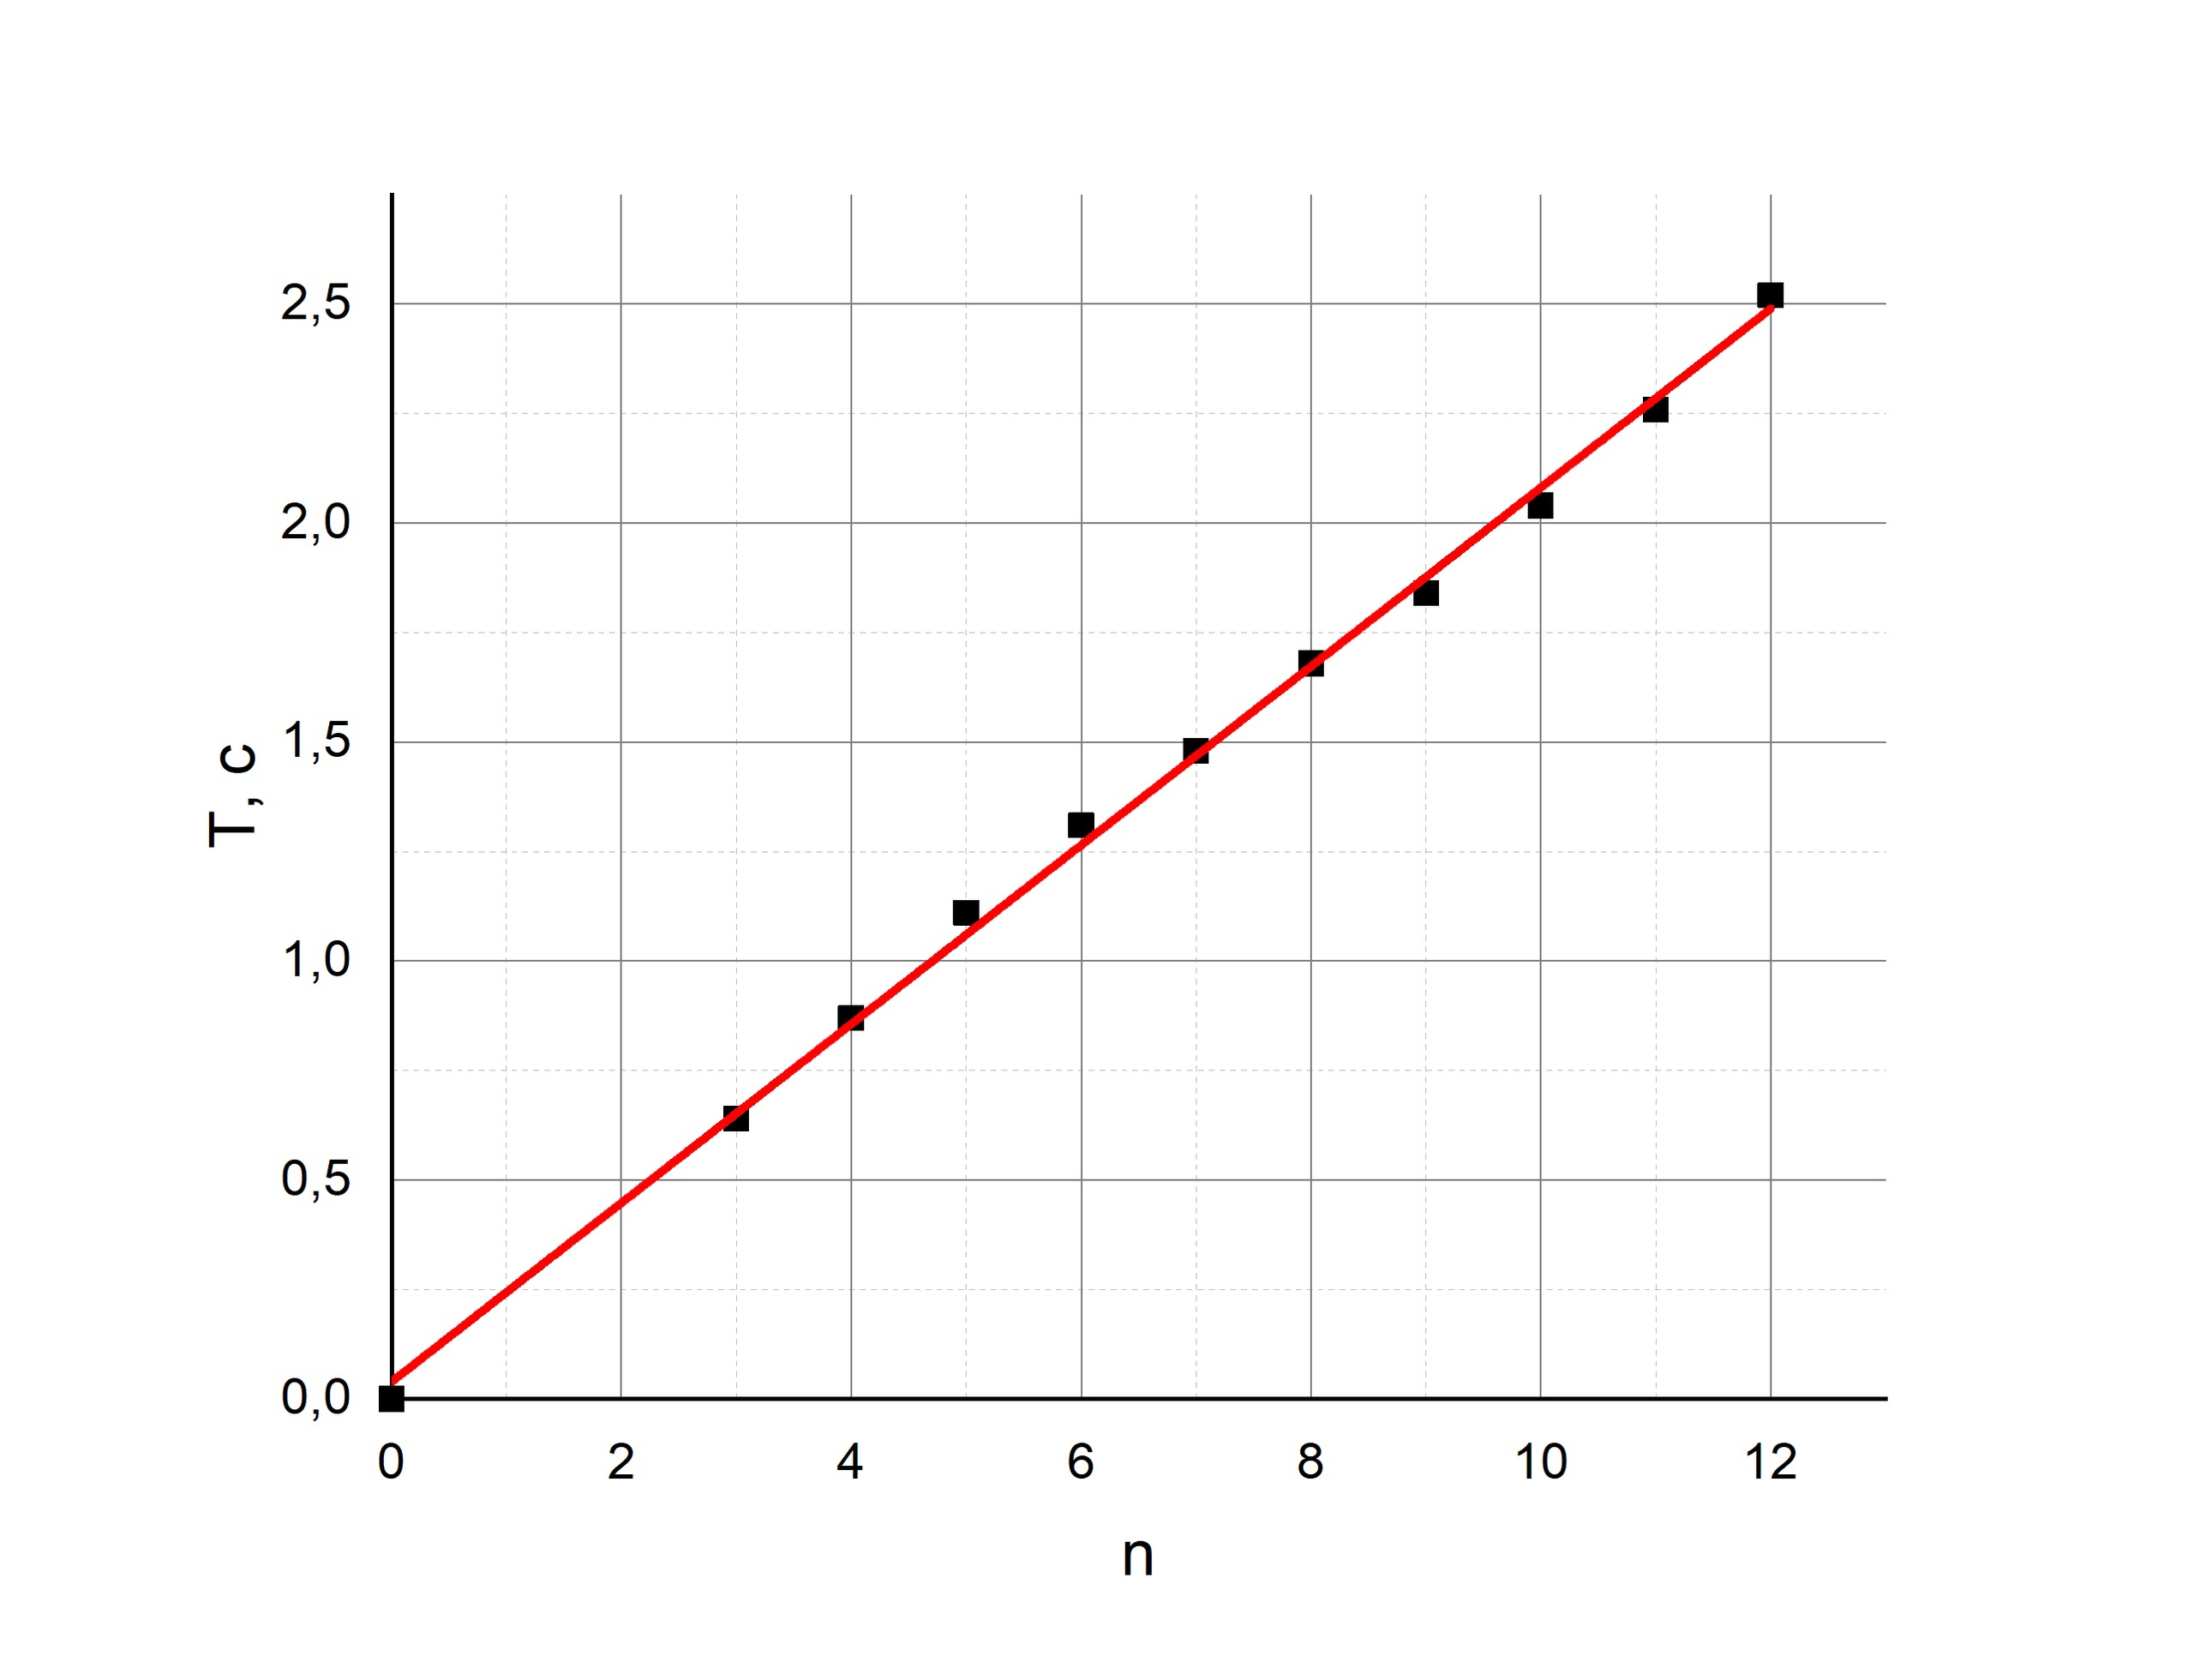
\includegraphics[width = 	15 cm]{graph1}
\caption{Зависимость Т(n)}
\end{center}
\end{figure}

Из МНК находим коэффициент наклона прямой:

$$
	k = 0,20 \pm 0,003 \ c
$$

Рассчитаем величину горизонтальной составляющей магнитного поля Земли по формуле:

$$
	B_{||} = \frac{\pi^2md^2}{3k^2 \mathfrak{m}} \approx 0,209 \ Гс
$$
$$
	\sigma_{B_{||}} = B_{||} \sqrt{\frac{\sigma_{\mathfrak{m}}^2}{\mathfrak{m}^2} + 4 \frac{\sigma_d^2}{d^2}} \approx 0,02 \ Гс
$$

\newpage

\subsection*{Задание №3}

\subsubsection*{Определение вертикальной составляющей магнитного поля Земли}

Изготовим <<магнитную стрелку>> из n = 10 шариков и подвесим её за середину.С помощью кусочков проволоки уравновесим <<стрелку>> в горизонтальном положении. Из условия равновесия рассчитаем механический момент сил M.Измерения проведем для четных значений n. Данные занесем в Таблицу 3.

\begin{table}[h]
\begin{center}
\caption{}
\begin{tabular}{|c|c|c|c|c|}
\hline
\textbf{M, дин*см} & 140,6474 & 175,8092 & 105,4855 & 82,96615 \\ \hline
\textbf{n}         & 10       & 12       & 8        & 6        \\ \hline
\end{tabular}
\end{center}
\end{table}

По данным Таблицы 3 построим зависимость M(n):

\begin{figure}[h]

\begin{center}

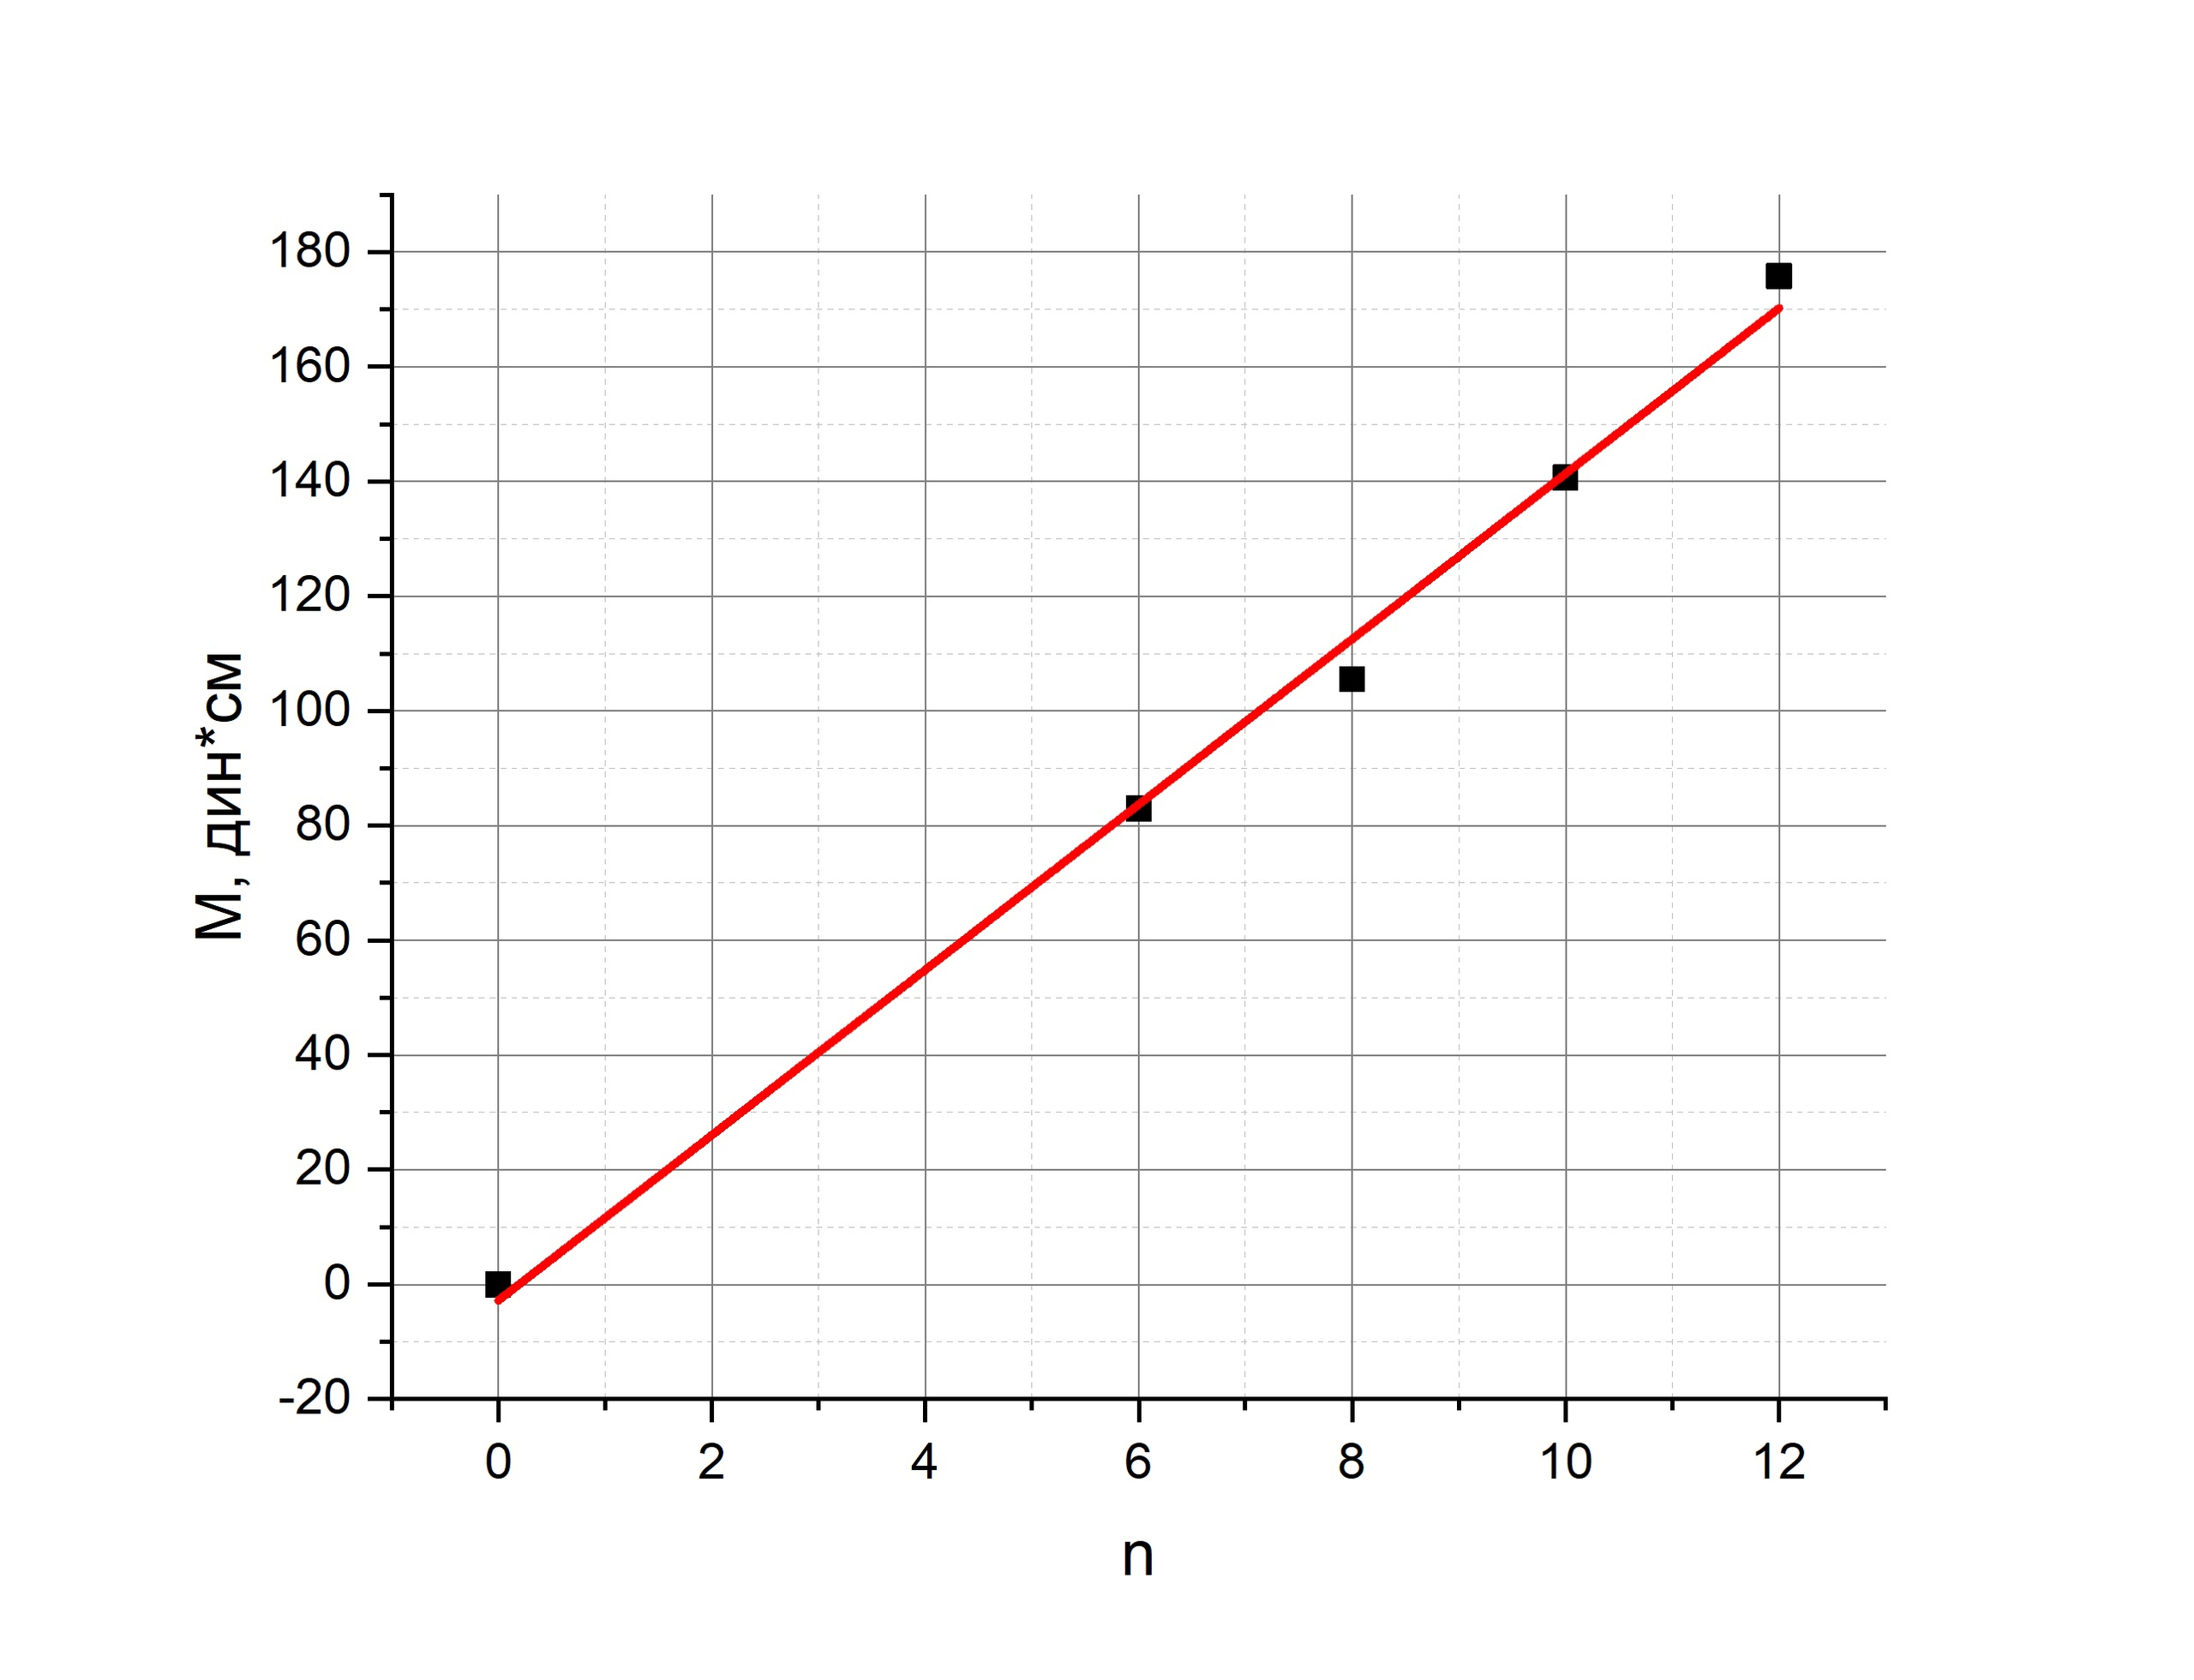
\includegraphics[width = 15 cm]{graph2}
\caption{Зависимость M(n)}
\end{center}
\end{figure}

Из МНК находим коэффициент наклона прямой:

$$
	A = 14,42 \pm 0,59 \ дин*см
$$

\newpage

По значению коэффициента наклона найдем величину вертикальной составляющей магнитного поля Земли по формуле:

$$
	B_{\perp} = \frac{A}{\mathfrak{m}} \approx 0,32 \ Гс
$$	
$$	 
	\sigma_{B_{\perp}} = B_{\perp} \sqrt{\frac{\sigma_{\mathfrak{m}}^2}{\mathfrak{m}^2} + \frac{\sigma_A^2}{A^2}} \approx 0,03 \ Гс
$$

Определим магнитное наклонение $\beta$:
$$
	\beta = \arctan \frac{B_{\perp}}{B_{||}} = 57 ^\circ
$$

$$
	\sigma_{\beta}^2 = \sqrt{\frac{\sigma_{B_{\perp}}^2 B_{||}^2 +\sigma_{B_{||}}^2 B_{\perp}^2} {B_{||}^2 (1 + \frac{B_{\perp}^2}{B_{||}^2})^2}} \approx 3^\circ
$$
Определим полую индукцию B Земли
$$
	B = \sqrt{B_{\perp}^2 + B_{||}^2} \approx 0,38 \ Гс	
$$
$$
	\sigma_B = \sqrt{\frac{\sigma_{B{||}}^2B_{||} + \sigma_{B{\perp}}^2B_{\perp}}{\sqrt{B_{\perp}^2 + B_{||}^2}}} \approx 0,03 \ Гс
$$

Окончательно
$$
	\beta = (57 \pm 3)^\circ
$$
$$
	B = 0,38 \pm 0,03 \ Гс
$$



\section{Выводы}


1)В результате работы было установлено, что более точное значение магнитного момента может быть получено методом Б, так как остаточная индукция поля, рассчитанная по методу Б, $B_r = 8922 \pm 553 \ Гс $, дает более близкое к теоретическому значению $B_r = 12 кГс$. Отклонения от теоретического значения могут быть вызваны неоднородностью поверхности шаров и, следовательно, неточно измеренными геометрическими размерами.

2)Также были получены значения для параллельной $B_{||} = 0,209 \pm 0,02 Гс$ и перпендикулярной $B_{\perp} = 0,32 \pm 0,03 Гс$ составляющих индукции магнитного поля Земли, а также рассчитано магнитное наклонение $\beta = (57 \pm 3)^\circ$ на широте Москвы. Все эти величины совпадают с теоретическими по порядку величины, однако не совпадают численно. Данное расхождение может быть связано с недостаточно точными вычислениями магнитных дипольных моментов 




\end{document}
